\documentclass[12pt]{scrartcl}
\usepackage{graphicx}
\usepackage{amsmath}

\newcommand{\RN}[1]{%
  \textup{\uppercase\expandafter{\romannumeral#1}}%
}

\usepackage{fourier} 
\usepackage{array}
\usepackage{makecell}

%\renewcommand{\arraystretch}{1.5}
%\renewcommand{\cellalign/theadalign}{cl}


\begin{document}
\title{Interaction of a "cold plume" with a subduction zone}
\subtitle{Semester Thesis}
\author{Florian Frei}

\maketitle

\newpage

\tableofcontents

\newpage

\section{Motivation}
Seismological measurements from Columbia shown in figure \ref{fig:seism_data} suggests that an rare geological scenario is happening. The geophysical community agrees that what is probably happening is the rare case where a "cold plume" is detached from the lithosphere and interacts with the subduction plate beneath it. In this project the goal is to use a simplified subduction model to simulate what longterm tendencies could develop and investigate the sensitivity on the parameters for the individual scenarios.
\begin{figure}
\includegraphics[scale=0.45]{deep_anomaly_hor_ver.png}
\label{fig:seism_data}
\end{figure}

\section{Geophysical Model}
The skill how to correctly model geophysics for a numerical simulation is to vast that it could fit into a single book much less into a simple report. A good starting point which is essential to understand this project is the book "Introduction to Numerical Geodynamic Modelling" \cite{gerya2009introduction} written by Taras Gerya. This project can also be seen as an additional example in application of geophysical numerical modeling.
\subsection{Physical Equations}
For completeness all equations used in the simulation are listed below. Most equations originate from the fact that the material is seen as a continuum. Therefore one can intuitively guess that the three conservation laws are used for describing its behavior. Namely the conservation of mass, momenta and energy or in this case heat. First the conservation of mass is described by the continuity equation written in Eulerian form as:
\begin{align}
\frac{d \rho}{d t} + \nabla \cdot (\rho \mathbf{v})&=0
\intertext{, and in the Lagrangian form as:}
\frac{D \rho}{D t} + \rho \nabla \cdot \mathbf{v}&=0
\end{align}
, where $\rho$ is the local density of the material and $\mathbf{v}=\begin{pmatrix}v_x\\v_y \end{pmatrix}$ the local velocity.\\
The second law, conservation of momenta, is described by the Navier-Stokes equations. Since this project is a model in two dimensions the reduced Naver-Stokes equation in Eulerian form is written as:
\begin{align}
\frac{\partial \sigma_{xx}'}{\partial x}+\frac{\partial \sigma_{xy}}{\partial y}-\frac{\partial P}{\partial x}+\rho g_x&=\rho \left( \frac{\partial v_x}{\partial t}+v_x\frac{\partial v_x}{\partial x}+v_y\frac{\partial v_x}{\partial y} \right)\\
\frac{\partial \sigma_{yy}'}{\partial x}+\frac{\partial \sigma_{yx}}{\partial y}-\frac{\partial P}{\partial y}+\rho g_y&=\rho \left( \frac{\partial v_y}{\partial t}+v_x\frac{\partial v_y}{\partial x}+v_y\frac{\partial v_y}{\partial y} \right)\\
\intertext{and in Lagrangian form as:}
\frac{\partial \sigma_{xx}'}{\partial x}+\frac{\partial \sigma_{xy}}{\partial y}-\frac{\partial P}{\partial x}+\rho g_x&=\rho \frac{D v_x}{D t}\\
\frac{\partial \sigma_{yy}'}{\partial x}+\frac{\partial \sigma_{yx}}{\partial y}-\frac{\partial P}{\partial y}+\rho g_y&=\rho \frac{D v_y}{D t}\\
\end{align}
Last but not least the third conservation law, conservation of heat, also known as temperature equation, can be derived from Fourier's law of heat conduction and has the following Lagrangian form, assuming $k$ is constant:
\begin{align}
\rho C_p \frac{D T}{D t} &= k (\frac{\partial^2 T}{\partial x^2}+\frac{\partial^2 T}{\partial y^2})+H_r+H_s+H_a+H_L\\
\intertext{or in Eulerian form:}
\rho C_p (\frac{\partial T}{\partial t}+v_x \frac{\partial T}{\partial x} + v_y \frac{\partial T}{\partial y})&= k (\frac{\partial^2 T}{\partial x^2}+\frac{\partial^2 T}{\partial y^2})+H_r+H_s+H_a+H_L
\intertext{In this project only two heating terms are considered relevant namely the adiabatic heating $H_a$ and the shear heating $H_s$. These two are approximated with the following relations:}
H_a &\approx \alpha\cdot T \cdot v_y \cdot \rho \cdot g_y\label{eq:ha}\\
H_s &\approx \sigma_{xx}\cdot \dot{\epsilon}_{xx} + \sigma_{xy}\cdot \dot{\epsilon}_{xy}\label{eq:hs}
\end{align}
All these equations have in common namely that they are all partial differential equations in space and time where mostly an analytical solution cannot be found. Furthermore to find a solution on a domain one requires additional information such as the initial state and boundary conditions. \\
With these tree equation one can depict how the continuum moves and how the temperature develops but what is still missing is the behavior of the material under these changes. This is defined in the rheology of rocks. There are a lot of possible choices for the behavior like visco-elastic, visco-plastic etc. to name just a few. In this project for simplicity we use a well-known empirical rheological relationship \ref{eq:emprheolrel} between strain-rate and differential stress which is of the following form:
\begin{equation}
\dot{\gamma}=A_D h^m (\sigma_d)^n\exp\left( -\frac{E_a+V_a P}{RT} \right)
\label{eq:emprheolrel}
\end{equation}
Note however that $A_D,h,E_a$ and $V_a$ are still parameters which have to be defined. A sensible choice will be shown in section \ref{seq:modelsetup} about the model setup. As already shown in equation \ref{eq:ha} and \ref{eq:hs} the standard definition of stress, strain and strain-rate are mandatory for the description.
\begin{align}
\sigma_{ij}'&=\sigma_{ij}+P\delta_{ij}\\
\sigma_{\RN{2}}&=\sqrt{\frac{1}{2}(\sigma_{ij}')^2}\\
\epsilon_{ij}&=\frac{1}{2}\left( \frac{\partial u_i}{\partial x_j}+\frac{\partial u_j}{\partial x_i}\right)\\
v_i&=\frac{D u_i}{D t}\\
\dot{\epsilon_{ij}}&=\frac{1}{2}\left( \frac{\partial v_i}{\partial x_j}+\frac{\partial v_j}{\partial x_i}\right)\\
\dot{\epsilon}_{ij}'&=\dot{\epsilon}_{ij}-\delta_{ij}\frac{1}{3}\dot{\epsilon}_{kk}\\
\dot{\epsilon}_{kk}&=\nabla \cdot \mathbf{v}\\
\dot{\epsilon}_{\RN{2}}&=\sqrt{\frac{1}{2}(\dot{\epsilon}_{ij}')^2}
\end{align}
Also the property for isotropic, incompressible materials \ref{eq:iim} will be utilized.
\begin{equation}
\sigma_{\RN{2}} = 2 \eta_{eff}\dot{\epsilon}_{\RN{2}}
\label{eq:iim}
\end{equation}

\section{Model setup}
\label{seq:modelsetup}
First of all the model setup for a subduction zone will be shown as a basis. This model is utilized for simulating the subduction of a slab from the lithosphere into the asthenosphere. Depending on the properties of the necking area different scenarios occur. The actual model of this project takes a segment of this model and places a "cold plume" above the slab. In this model the interest lies not in the process of breaking of the slab but in the interaction between the slab and the plume where different tendencies develop.
\subsection{Model of a subduction zone}
The model of a subduction zone consists of three layers. Namely the water layer, the lithosphere and the asthenosphere. These layers are shown in figure \ref{fig:modelsubductionzone}. The green section describes the necking are which determines the development of the simulation. To get a complete problem the parameters and rheology has to be characterized for all layers in addition also the initial state and boundary conditions have to be chosen. A standard model is described as follows:\\
\begin{tabular}{lll}
layer&property&value\\
water&&\\
&density $\rho$&$1000 [\frac{kg}{m^3}]$\\
&temperature $T$&$273[K]$\\
&viscosity $\eta$&$10^{18} [Pa\cdot s]$\\
&thermal conductivity $k$&$300 [\frac{W}{m\cdot K}]$\\
&heat capacity $C_p$&$3000 [\frac{J}{kg\cdot K}]$\\
&thermal expansion $\alpha$&not needed$[\frac{1}{K}]$\\
&compressibility $\beta$&not needed$[\frac{1}{Pa}]$\\
&stress strength $\sigma_{yield}$&not needed$[\frac{J}{m^3}]$ \\
lithosphere&&\\
&density $\rho$&$3300 [\frac{kg}{m^3}]$\\
&temperature $T$&$T(y) [K]$\\
&viscosity $\eta$&$10^{23} [Pa\cdot s]$\\
&thermal conductivity $k$&$k(T) [\frac{W}{m\cdot K}]$\\
&heat capacity $C_p$&$1000 [\frac{J}{kg\cdot K}]$\\
&thermal expansion $\alpha$&$3\cdot10^{-5}[\frac{1}{K}]$\\
&compressibility $\beta$&$10^{-11}[\frac{1}{Pa}]$\\
&stress strength $\sigma_{yield}$&$5\cdot 10^7[\frac{J}{m^3}]$ \\
asthenosphere&&\\
&density $\rho$&$3250 [\frac{kg}{m^3}]$\\
&temperature $T$&$1500 [K]$\\
&viscosity $\eta$&$10^{19} [Pa\cdot s]$\\
&thermal conductivity $k$&$k(T) [\frac{W}{m\cdot K}]$\\
&heat capacity $C_p$&$1000 [\frac{J}{kg\cdot K}]$\\
&thermal expansion $\alpha$&$3\cdot10^{-5}[\frac{1}{K}]$\\
&compressibility $\beta$&$10^{-11}[\frac{1}{Pa}]$\\
&stress strength $\sigma_{yield}$&$5\cdot 10^7[\frac{J}{m^3}]$ \\
\end{tabular}

\begin{align}
T(y) &= \frac{(1500 - 273)}{50} \cdot (y - 50) + 273\\
k(T) &= 0.73 + \frac{1293}{T+77}\\
\rho(\beta,\alpha,P,T)&=3300\cdot \frac{1+\beta \cdot (P-P_0)}{1+\alpha \cdot (T-T_0)}\\
\epsilon_{\RN{2}}&=\sqrt{0.5\cdot(\dot{\epsilon}_{xx}^2+\dot{\epsilon}_{yy}^2)+\dot{\epsilon}_{xy}^2 }\\
\eta(A_D,n,V_a,E_a,T,P,\epsilon_{\RN{2}})&=\frac{0.5}{A_D^{\frac{1}{n}}}\cdot \epsilon_{\RN{2}}^{\frac{1}{n}-1}\cdot \exp{\frac{(E_a+P\cdot V_a)}{R\cdot T \cdot n}}
\end{align}

\begin{tabular}{llll}
rock type&parameter&value&zone\\
dry olivin&&&lithosphere and slab\\
&$A_D$&$2.5\cdot 10^{-17}$&\\
&$n$&$3.5$&\\
&$V_a$&$8\cdot 10^{-6}$&\\
&$E_a$&$532000$&\\
wet olivin&&&asthenosphere\\
&$A_D$&$2\cdot 10^{-21}$&\\
&$n$&$4$&\\
&$V_a$&$4\cdot 10^{-6}$&\\
&$E_a$&$471000$&\\
\end{tabular}

\begin{figure}
\includegraphics[scale=0.8]{model1.pdf}
\caption{model structure of subduction zone}
\label{fig:modelsubductionzone}
\end{figure}

\begin{tabular}{ll}
constant&value\\
universal gas constant $R$&$8.314$\\
viscosity cutoff $\eta_{min}$&$10^{16}$\\
viscosity cutoff $\eta_{max}$&$10^{24}$\\
standard temperature $T_0$&$273[K]$\\
standard pressure $P_0$&$10^5 [Pa]$\\
\end{tabular}\\

At this step the model description for the initial state, the rheology and the constants are all defined. What is missing is the boundary condition used for solving the temperature and Navier-Stokes equations. For the Navier-Stokes solver there many possible choices but only two are presented here. These are the no slip and free slip boundary conditions.\\ 

\begin{tabular}{ll}
boundary condition&property\\
no slip&$v_x=0$ and $v_y=0$ everywhere on the boundary\\
free slip&\makecell[l]{ $\frac{\partial v_y}{\partial x}=0$ and $v_x=0$ on boundaries parallel to y-axis\\$\frac{\partial v_x}{\partial y}=0$ and $v_y=0$ on boundaries parallel to x-axis }
\end{tabular}
%$\frac{\partial v_y}{\partial x}=0$ and $v_x=0$ on boundaries parallel to y-axis\newline$\frac{\partial v_x}{\partial y}=0$ and $v_y=0$ on boundaries parallel to x-axis\\
For the temperature equation first of all a linear gradient in the lithosphere was chosen from $273K$ to $1500K$ which is also present in the slab. For the top and bottom boundary which are parallel to the x-axis a constant heating boundary condition was selected with $273K$ and $1500K$ respectively. For the left and right boundary parallel to the y axis thermal insulation was the most sensible choice, meaning the temperature is set equal to the temperature from the neighboring grid point on the right/left.\\

Since the solvers for the Navier-Stokes and temperature equations work only on discrete grids the model is also solved only on the grid points. Therefore the choice of how the grid is defined influences the whole simulation process. In this project the same staggered grid as explained in \cite{gerya2009introduction} was used. Thus the properties are fixed on material points like in the Lagrangian view which will be interpolated on to the fixed grid which will be shortly explained in the implementation section \ref{seq:impl}.

\subsection{Model of this project}
Now the actual domain of this project refines the above model on to a smaller domain with an additional "cold plume" as roughly indicated with the white borders in figure \ref{fig:modelsubductionzone}. The new model is shown in figure \ref{fig:tm}. Therefore all previously mentioned properties, constants and equations can be transfered on to the new model but note that some are slightly modified which will be listed next. Since there is no longer a water layer these properties can be ignored in this model and the properties of the "cold plume" has to be added which are the following:\\
\begin{tabular}{lll}
plume&&\\
&density $\rho$&$3500 [\frac{kg}{m^3}]$\\
&temperature $T$&$700 [K]$\\
&viscosity $\eta$&$10^{23} [Pa\cdot s]$\\
&thermal conductivity $k$&$k(T) [\frac{W}{m\cdot K}]$\\
&heat capacity $C_p$&$1000 [\frac{J}{kg\cdot K}]$\\
&thermal expansion $\alpha$&$3\cdot10^{-5}[\frac{1}{K}]$\\
&compressibility $\beta$&$10^{-11}[\frac{1}{Pa}]$\\
&stress strength $\sigma_{yield}$&$p_3 [\frac{J}{m^3}]$ \\
\end{tabular}

Since the goal of this project is to see the different tendencies of this setup $\sigma_{yield}$ is varied as a parameter $p_3$. $p_3$ is assigned to take on $10^7$, $2\cdot 10^7$, $5\cdot 10^7$, or $10^8$. The first parameter $p_1$ is the actual starting position of the plume $(x_p,y_p)$ marked as yellow in figure \ref{fig:tm}. This position was varied across three types. First where the plume has not much space on the left side and is near the contact point with the slab. Second in the middle of the slab where enough space is on both sides and the contact point is near or far away. And lastly the third position is near the edge of the slab and has the most distance to the contact point.
The second parameter $p_2$ is the angle $\gamma$ of the slab shown in green. The angle was chosen to be $20$, $30$, $45$ or $60$ degree. The forth parameter $p_4$ is $\sigma_{yield}$ of the buffer zone marked as bright blue in figure \ref{fig:tm}. This can take on the same values as $p_3$. The last and fifth parameter $p_5$ of the model is the radius of the plume indicated as white in figure \ref{fig:tm}. The radius is assigned to be $10$, $15$, $20$, $25$ or $30$ kilometers. A vigilant reader can guess that the number of simulations can exceed $1000$ possibilities. Therefore only different tendencies are reported in the results section. The code of this project will be online obtainable for the interested reader to try different simulations himself. A warning is here issued since one simulation can take up to $30$ minutes and it is not guaranteed that all quantities remain physically meaningful since numerical errors amplify with time.

\begin{figure}[!ht]
\includegraphics[scale=1.2]{model2.pdf}
\label{fig:tm}
\caption{model of this project}
\end{figure}



\section{Implementation}
\label{seq:impl}

flow diagram

\section{Results}
\section{Conclusion}

\nocite{vargas2013tearing}
\nocite{gerya2009introduction}




\newpage

\bibliographystyle{plain}
\bibliography{references}


\end{document}

